\documentclass[Journal,letterpaper, NoLineNumbers]{ascelike-new}
%% Please choose the appropriate document class option:
% "Journal" produces double-spaced manuscripts for ASCE journals.
% "NewProceedings" produces single-spaced manuscripts for ASCE conference proceedings.
% "Proceedings" produces older-style single-spaced manuscripts for ASCE conference proceedings. 
%
%% For more details and options, please see the notes in the ascelike-new.cls file.

% Some useful packages...
\usepackage{booktabs}
\usepackage{dcolumn}
\usepackage[utf8]{inputenc}
\usepackage[T1]{fontenc}
\usepackage{lmodern}
\usepackage{graphicx}
\usepackage[figurename=Fig.,labelfont=bf,labelsep=period]{caption}
\usepackage{subcaption}
\usepackage{amsmath}
%\usepackage{amsfonts}
%\usepackage{amssymb}
%\usepackage{amsbsy}
\usepackage{epigraph}
\usepackage{newtxtext,newtxmath}
\usepackage[colorlinks=true,citecolor=red,linkcolor=black]{hyperref}
%
% Please add the first author's last name here for the footer:

% Note that this is not displayed if the NoPageNumbers option is used
% in the documentclass declaration.
%
\begin{document}

% You will need to make the title all-caps
\title{ Refining Tastes:\\
Analysis of Preference Formation Models on Asian Cuisines}

\author[1]{Lindsey Currier, Jonathan Greenberger, Eric Li, Johnny Ma, Kevin Tse \\ University of Chicago\footnote{We thank Sebastien Gay and Kyle Kost for being great teachers and giving us the methods to run these regressions. Special Thanks to Jim Marrone (Ph.D. candidate, Economics) and Jonathan Dingel (Assist. Professor, Chicago Booth) for help in conceptualization and methodology. Thanks to Colin Camerer, Melissa Tartari, Sylvia Klosin, and Cameron Taylor for general advice.}}
\maketitle
 % Refining One's Palate: Something something  how tasty foods  form one's taste 



\begin{abstract}
We develop and test \textit{habit formation} and \textit{learning-by-consumption} models of preference formation of Asian cuisines. Using user-generated data provided by Yelp, we study the effect of past experience on a consumer's current demand for a particular type of food, here Asian. Specifically, we study the effect of \textit{initial experience} with this cuisine on the formation of habit and taste, which earlier studies were unable to investigate due to limitations in data.  We do not find a positive correlation between initial experience with a cuisine and an agent's future consumption of the same cuisine, a result that does not substantiate the \textit{learning-by-consumption} model. We further look at the effect of previous consumption on current consumption. Here we find that consumption in one period of a new cuisine and consumption in the next period of the same cuisine are positively correlated, suggesting that preference for food may be driven by habit.
\end{abstract}

\section{Introduction}
 
Preference theory and taste formation are areas in which both theoretical and empirical studies are sorely lacking. Though agents' preferences are formed over time, many standard economic models take them to be given at every moment without initial formation of those preferences and their subsequent evolution. One area of consumption rife with opportunities for this type of analysis is food. Both a basic good required by everyone and highly multifaceted, food can be considered a cultural good, as each cuisine is closely associated with people's tastes, habits, and cultural identities. As a result, consumers' preferences for different kinds of food are formed and change over time as they gather more experience with said cuisine. However, the effect of past experience, most notably the initial experience, on future consumption is unclear. One might think a good first experience with Thai food would create a long time Thai food lover, but how strongly does that instance impact future decisions? Conversely, a poor first experience might either prompt an individual to attribute the bad taste to the cuisine type or to the restaurant itself, which would lead to no more future visits or an almost guaranteed future visit respectively. 

Three notable models have been proposed to explain taste formation. They are, specifically, the \textit{habit formation theory} outlined by Houthakker and Taylor (1970) and Pollak (1970), the \textit{learning-by-consumption theory} outlined by Levy-Garboua and Montmarquette (1996), and the classical \textit{rational addiction} framework developed by Becker and Stigler (1977). These models, and their mixtures and variants, have been applied to numerous types of preference-inconsistent goods, such as theater (Castiglione and Infante, 2016), cinema (Yamamura 2008), language (Marrone, forthcoming), and cigarettes (Becker et al., 1994).

We are interested in using these models to answer the question of how preference for food consumption is formed with a causal argument. In addition, we seek to study how initial exposure to a new type of cuisine, specifically Asian cuisine, informs future consumption behaviors of the same, or related, cuisines. We focus on Asian cuisine because it is a branch of cuisine that is relatively popular in America, ensuring a good sample size, but is still uncommon enough to find initial users. In addition, many Asian restaurants draw from multiple ethnicities (i.e. Chinese restaurant serving Japanese sushi). Our data set is 2.2 million reviews from the Yelp Dataset Challenge which contains individual level  user and restaurant characteristics, quantifiable scores and times of visit, and, uniquely, the text of reviews. This allows us to identify a user's point of initial exposure to a type of cuisine, enabling us to examine the effect of initial exposure on future consumption, a feat unprecedented in the literature. Insight into taste formation and evolution can be invaluable to businesses interested in attracting and maintaining a customer base. Additionally, our approach is likely generalization to all types of food experience and could inform us of preference formation of cultural goods. 

\section{Theory}
Three theories have been proposed to model preference formation as a function of past experiences.

The \textit{habit formation} theory, initially formulated by Houthakker and Taylor (1970) to explain consumer demands in the U.S., and expanded on by Pollak (1970), proposes that preferences are formed by habit. In this model, the consumer experiences a utility loss when current period consumption deviates from previous consumption. Therefore, the demand for a certain good ($D_{t}$) is directly influenced by consumption of the same good in the not-too-distant past, ($D_{t-1}$). As in the standard demand functions, the current price of the good ($P_{t}$), and income of the agent ($I_{t}$), also influence consumption behaviors. Certain consumer characteristics and good-specific traits are also controlled for. The model may be summarized with the following linear regression:
\[D_{t} = \beta_0 + \beta_1D_{t-1} + \beta_2P_{t} + \beta_3I_{t} + X'\gamma + U_t\]

Here, $X'$ represents the vector of control variables and $U_t$ is the errors not explained by the econometrician.  This model implies that a change in price or income may cause a change in consumption, which induces a change in preferences for the next period through the formation of habit, in turn leading to further changes in consumption in the following periods. Note that while consumption in the distant past is not a regressor, it is incorporated into the model as $D_{t-1}$ is itself influenced by $D_{t-2}$, and so on. To more directly incorporate the past, one could run a similar regression on a weighted average of consumption in all previous periods. Furthermore, this model does not treat agents as forward-looking, as they do not take into consideration the impact of current consumption on future shifts in taste and demand. Previous papers have sought to explain demand for food using the habit formation model, including Pope, Green, and Eales (1980), which uses macro data to study economy-wide demand of meat, and Heien and Durha (1991), which explores people's decision to go to restaurants.  

The second theory, \textit{learning-by-consumption}, was first proposed by Levy-Garboua and Montmarquette (1996) to study the demand for theater. In this model, consumers discover their pre-existing, but unknown, preferences through repeated consumption of a good in a sequential, learning process. Every time an agent consumes, they experience either a positive or negative "surprise." These "surprise" shocks accumulate into experience, $S_t$, which influences their demand for a good in the next period. The \textit{learning-by-consumption} model takes into account both new experience ("the shock," $\epsilon_t$) and all past experiences ($S_{t-1}$). This is weighted by a decay of memory ($1-\delta$) that depends on how recent the past period consumption was. The model for accumulated experience, $S_t$, may be simplified down to the basic autoregressive model:
\[S_t = (1-\delta)S_{t-1} + \epsilon_t\]

The overall model can be written as
\[D_{t} = \beta_0 + \beta_1S_{t} + \beta_2P_{t} + X'\gamma + U_t\]

It is important to recognize that \textit{learning-by-consumption}, like \textit{habit formation}, is not forward looking; agents do not maximize life-time utility because they do not take into consideration the effect of changing preferences in the current period on future consumption, as they do not know what the preference "shock" will be until it has occurred. 

In contrast, the third theory, \textit{rational addiction} (Stigler and Becker 1977; Becker and Murphy 1988) considers agents as consistently forward looking. This framework has been used to show that given certain preferences, an agent might be acting rationally when they engage in a an addictive activity, such as smoking. In the model, current utility is affected by "consumption capital," or the extent of addiction, which is built-up over time through repeated consumption over periods. Agents take into account the effect of current consumption on consumption capital, which affects anticipated future consumption. Then, they act rationally by maximizing their lifetime utility, behaving in the present with consideration of all periods, past, present, and future.  A simple forward looking model (in which agent only looks forward one period) that can be generalized to take all future periods into account can be written as follows: 
\[D_{t} = \beta_0 + \beta_1D_{t-1} + \beta_2D_{t+1} + \beta_3P_{t} + \beta_4I_{t} + \beta_5P_{t+1} + \beta_6I_{t+1} + X'\gamma + U_t\]

Here, the rational expectation model is used where consumers project future incomes and costs of a good, and chooses current consumption accordingly. 

\section{Models}

Despite the obvious rigor of the \textit{rational addiction} theory, we do not use this model for several reasons. Firstly, we have no data before 2006 or after 2015, which prevents us from modeling lifetime behaviors by agents. Secondly, food, unlike goods such as cigarettes and theater, is arguably less addictive in the sense that individuals often do not take into account long term future consumption when deciding where to eat and how much they enjoy a certain cuisine. In contrast, cigarette consumption intuitively demands more future consideration due to health concerns. Hence, we will focus on the \textit{habit formation} and \textit{learning-by-consumption} models.

The \textit{habit formation} model assumes that the magnitude of the preference formation effect in each period is persistent; that is, the effect of past consumption on current consumption is of the same linear magnitude regardless of the time subscript. In other words, if exogenously increasing consumption in period 1 by one unit leads to two additional consumption units in period 2, then an increase in period 10 by one unit leads to two additional consumption units in period 11. The \textit{learning-by-consumption} model, likewise, faces the same problem, as a marginal shock of consumption knowledge increases next period consumption by the same amount at any point in time, regardless of how much previous exposure the consumer has had to the good. Furthermore, it discounts via "decay of memory" the effect of past experiences on current consumption by time. Hence, initial impression has the least effect on consumption than all other experiences. This seems inadequate; a consumer's early consumption ("first impression") of a type of food probably has a greater effect on her eating habits than, say, her 30th consumption. Essentially, the consumer is likely to learn more about her preferences the first time she tries a new food than the 30th. Indeed, the effect might plateau at a certain point, where new experiences, either negative or positive, barely affects preferences. Due to lack of data, earlier papers are not able to study the effect of "initial experience," however, Yelp data allows us to pinpoint first consumption (see Data and Methodology for details). Our first set of models uses this information to study the effects of an initial experience (in $t=0$) of a particular cuisine, on the period immediately following this first experience ($t=1$). 

Our first model is based on \textit{learning-by-consumption}. We assume that a user's initial rating, $R_{0}$, of his first visit to a new type of Asian food, e.g. Thai, is accurately reflective of his experience. To determine if this is a positive or negative "surprise," we also determine this user's average rating of Asian restaurants prior to this visit, which can be said to approximate their expectations of all Asian food up to that point. The difference between the new rating, $R_0$, and this average, is called $\rho_0$, which reflects a surprise shock in preference due to initial consumption of a new cuisine. Note that $\rho_0$ is a binary variable: it is coded as 1 for a positive shock, and 0 for a negative shock. We propose a method of examining the \textit{learning-by-consumption} theory by the use of a probit model, regressing on the probability of return to an Asian restaurant based on initial shock. Let $Y_1$ be a binary variable, where $1$ represents the consumer returning to same type of Asian cuisine in future, and $0$ represents not returning to the same type of Asian. For example, if the initial experience was at a Thai restaurant, $Y_1$ would have a value of 1 if, after the initial experience, the individual reviewed another Thai restaurant, 0 if not. If return is positively correlated to a positive knowledge shock, the regression supports the model. Clearly, if a consumer decides not to revisit a cuisine, there's no restaurant characteristics to control for and the probit model is unaffected. Thus, we only control for location of the restaurant. There are six American cities, as well as Quebec, considered as locations, based on all available Yelp data for those who had an initial experience. We use six location dummies as is standard, in order to avoid linear dependence issues. We then obtain the following linear model: For some $U \sim N(0,1)$, we say    
\[Y_1 = \begin{cases}
                        1, \text{if }\beta_0 + \beta_1\rho_{0} + \gamma_4C_1 + ... + \gamma_9C_6 + U > 0 \\
                        0, \text{ if otherwise}
                    \end{cases}\
\]

Let $\Phi$ be the standard normal distribution function. Then this linear regression can be rewritten into the probit model
\begin{equation}
\Pr(Y_1 = 1) = \Phi(\beta_0 + \beta_1\rho_{0} + \gamma_4C_1 + ... + \gamma_9C_6)
\end{equation}

We also examine a variation of this \textit{learning-by-consumption} model. Instead of investigating whether a first-time consumer of a type of Asian cuisine returns to that particular cuisine, we study if the initial experience affect his decision to visit Asian restaurants in general. This formulation thus treats Asian cuisine as similar, where a shock in one type of particular Asian cuisine might change people's going behavior towards Asian cuisine in general. Here, we seek to investigate if American consumers in the six cities we studied, as well as Quebec. We define $Y_2$, a binary variable, as whether a consumer visits any Asian restaurant after an initial visit to a particular type of Asian cuisine. The rest of the probit model is similar to the preceding one.
\begin{equation}
\Pr(Y_2 = 1) = \Phi(\beta_0 + \beta_1\rho_{0} + \gamma_4C_1 + ... + \gamma_9C_6)
\end{equation}

Our third model, based on \textit{habit formation}, differs from that used by Castiglione and Infante only in the specificity of time-frame that we selected. At the time of consumption of a new cuisine, no previous habit has been formed, so we cannot study consumption behavior prior to the time of the first experience. We instead focus on the period immediately following that initial experience. We select users who ate a type of Asian cuisine for the first time in our initial time period. We take this initial time frame as period $t-1$ and following year as period $t$. We assume that restaurant going habits form at some level within one year. Within this study, we set the initial year as 2014, and the following year as 2015. This is due to data considerations. Let $D_{2015}$ be the number of visits a consumer makes to the same cuisine in 2015, and $D_{2014}$ be number of visits in year 2014. We control for restaurant characteristics that may contribute to fixed effects including average prices of all Asian restaurants of interest a consumer visited in 2015 ($P_{2015}$), average quality of the same restaurants ($Q_{2015}$) and the six possible American cities in which the restaurants we examine are located, as well as Quebec, ($P, Q, C_1, ..., C_6$, respectively. We then obtain the following linear model: 
\begin{equation}
D_{2015} = \beta_0 + \beta_1D_{2014} + \gamma_1P_{2015} + \gamma_2Q_{2015} + \gamma_4C_1 + ... + \gamma_9C_6 + U_{2015}
\end{equation}

As our forth model, we run a different version of this "number of visits" model, but replace consumption in 2014, $D_{2014}$, with initial rating. This deviates from the \textit{habit formation} model and returns to a \textit{learning-by-consumption} model, as we are again using the "shock" of the initial experience. In this case, we are regressing number of visits on consumption shock, whereas in the probit model we are regressing likelihood to visit again on it. Thus, we regress consumption behavior in the period immediately following the initial exposure, year 2015, and obtain the following model: 
\begin{equation}
D_{2015} = \beta_0 + \beta_1\rho_0 + \gamma_1P_{2015} + \gamma_2Q_{2015} +  \gamma_4C_1 + ... + \gamma_9C_6 + U_{2015}
\end{equation}

\Section{Data and Methodology}
Our data is derived exclusively from round 7 of the "Yelp Data Challenge," which provided 2.2M reviews by 552K users for 77K businesses, written between 2006 and 2015. See table 1 for further summary user statistics\footnote{The R codes for \href{https://gist.github.com/anonymous/052c65ac01943dafe782415f2ce10e61}{Data Cleaning} and \href{https://gist.github.com/anonymous/0e4b6a6b6dd88b0e0c6e55794226ee07}{Regression} are linked here.}. We isolated our data to 6 American cities and Quebec, namely Pittsburgh, Charlotte, Urbana-Champaign, Phoenix, Las Vegas, Madison, and Quebec. We isolated restaurants to only Asian cuisine, which we defined as Chinese, Indian, Japanese, Korean, Mongolian, Thai, and Vietnamese. We focused on Asian cuisine because it offers the two qualities we need. First, it provides a relatively large sample size of reviewers across cities. Secondly, some users will be unfamiliar with aspects of Asian cuisine as it is non-native to our selected cities, enabling these users to still learn about their preferences for Asian food. Though it can be said that considering all Asian food under one category is problematic, both socially and statistically, many Asian restaurants serve multiple types of cuisine. Especially in America, many restaurants serve a type of Fusion Asian cuisine, which can be considered somewhat homogenous within the group "Asian." Although we considered using other ethnic food or alternatively all types of food, we found only a few instances of initial users in these cases. Thus, Asian foods were the perfect meeting of desirable qualities. 

An important assumption we make is that each reviewer submits a review for every restaurant they visit. This is necessary in order to make sure that a review equates a visit. Thus, we furthered isolated the data by selecting only "chronic reviewers" who wrote over thirty reviews between years 2014 and 2015. This relaxes the assumption of the total reviewer, we equate a "chronic reviewer's" number of visits to a particular cuisine with their numbers of reviews of that type of restaurant. 
Equating number of reviews with number of visits is a rather strong assumption, even when only "chronic reviewers" are considered. "How Segregated is Urban Consumption?" (Davis, Dingle, Monras 2016), a paper which also uses Yelp data, addresses this issue in depth. We will outline their explanation here. The paper initially assumes that the probability a user reviews a restaurant after a visit is constant, and unrelated to restaurants characteristics. So long as this is the case, they show that none of the estimated parameters will be biased. This assumption, however, might be unrealistic, as people may be more inclined to review more well known restaurant (or, equally likely, less well known restaurants). Nevertheless, even if the probability of review depends on characteristics of the restaurant, the paper shows that the regression only biases those parameters that depend on restaurant characteristics. As our parameter of interest depends on past visits, our regression won't be additionally biased so long the probability of review does not depend on previous reviews of that food type. Therefore, we need only assume that a regular Yelp user's decision to review a restaurant does not depend on past experiences with this general cuisine, a far weaker assumption. Essentially, this is stating that users do not grow tired of reviewing a certain type of cuisine just because they have reviewed it in the past, which seems to be a reasonable assumption for chronic reviewers.

A few other assumptions we make about our data include that reviewers are inhabitants of the city they live in, users do not re-review restaurants, and the day of review is the same as day of visit. From manual examination of data, we believe that these assumptions are mostly accurate. The day of review assumption is negligible as we are aggregating over year long time periods.

After isolating "chronic reviewers", we further isolate reviewers for whom the review indicated that had a first time eating at a specific Asian cuisine within our initial time frame. To obtain this information, we parse the "chronic reviewer" data and searched for instances within reviews where users explicitly indicated that their visit is their first exposure to a particular cuisine. Reviews with certain identifying phrases, such as "first time eating" or "never had before", were identified via a string-searching algorithm in R. These reviews were then manually reviewed, and false positives, such as "If you've never had Indian food before, this restaurant is ..." or "it was my mother's first time..." were eliminated from our data.

We further subset the data by only considering initial exposures that occur in the years 2013 and 2014. This is done because we want to focus on a period of time when Yelp is relatively popular, which is evidenced by the vast majority of reviews being post 2013. We use these years as they are before 2015, and thus the shock will supposedly be realized in the year 2015, the following period. Ideally, we would use only 2013 shocks, but we include 2014 shocks in order to add more points to our data set, and consider 2012 to be too distant from 2015, causing the decay to become likely highly significant. Though this consideration does not matter for habit formation, it does matter for our probit models that include shock.

In our model, each $D_{t,i}$ represent a consumer's consumption of a particular cuisine in time $t$ (i.e. the number of reviews submitted by a "chronic reviewer" in this time for a particular cuisine). $R_{0,i}$ represent user rating of an initial visit to a new cuisine. Each Yelp rating is is based on a five-star system, with half star increments (i.e. the lowest score greater than 3 stars is 3.5 stars). We also find the average rating of all Asian restaurants a user has reviewed up to the point of initial exposure to a new cuisine. This can be considered the average expectation that the user has for Asian food, up until the initial exposure point. We subtract this average from $R_{0,i}$ to obtain $\rho_{0,i}$, the "surprise" of the new cuisine. We don't regress directly on $R_{0,i}$ but use "surprise" because we are concerned with new knowledge, i.e., what the user "learned" through the new experience. $\rho$ is hence an exogenous preference shock. Moreover, subtracting average ratings from $R$ also helps us control for an user's overall rating behavior for Asian restaurants, which is necessary because some users may be harsher than others and tend to assign more or less stars to restaurants in general. In addition, for users who had not reviewed any Asian restaurants prior to their initial experience, we set their $\rho$ value to be their initial rating subtracted from the average rating of all Asian restaurants, which we take as the general expected rating of an Asian restaurant trip.

In addition to these parameters of interest, we also seek to control for a wide variety of consumer and restaurant characteristics that may contribute to fixed effects. For restaurant characteristics, we control for price, quality, and location. Price, $P_t$, is the average price of all restaurants that each consumer visits in period $t$. To determine price for each restaurant, we use the number of dollar signs they are assigned to by Yelp. Under this system, numbers of dollar signs represent approximate cost per meal per person at a certain restaurant, with \$ representing under \$10, \$\$, \$11-\$30, \$\$\$, \$31-\$60, and \$\$\$\$, above \$61. We assume this to be an accurate classification of price tiers, and assign a value of "1" to \$, "2" to \$\$, and so on. Note that Yelp only provides the current price of each restaurant, hence we must assume that price is constant over time. This is a relatively safe assumption given our short time frame. For users who did not visit new restaurants in period $t$, we assume that $P_t$ is equal to the price of the restaurant where the user had the initial experience with the cuisine. Here, we simply assume that users make decision based on past experience. Quality, $Q_t$, is the average of aggregate ratings of all restaurants a consumer visited in period $t$. The aggregate Yelp rating is simply the average of all Yelp  ratings, using the aforementioned five-star system, of a particular restaurant. We assume that this is an objective reflection of a restaurant's quality. Once again, Yelp only provides current aggregate rating for restaurants, thus we assume that the qualities of restaurants are constant over time. Note that both of these controls only look at the Asian restaurants that each individual visits in the time frames, which is then averaged to produce the average price and average quality. The mean  is the most intuitive way to aggregate and control for the characteristics of visited restaurants. 

For users who did not visit new restaurants in period $t$, we assume that $Q_t$ is equal to the average quality of all Asian restaurants in our list. We used the same process to fill in for $P_t$. Lastly, we control for the location of the restaurant by assigning dummy variables $C_1, ..., C_6$ for the cities we examine, where we have one less . Controlling for city captures all location fixed effects, such as difference in GDP per capita growth across different regions, and different food popularity trends. We also note the supply of Asian restaurants in our data ranges goes from 172, 169 and 162 from 2013, 2014, and 2015 respectively. Thus, we can say that changes in supply should have negligible effects on consumption patterns, given the relatively stable number of Asian restaurants. 
	
    We test for heteroskedasticity in all of our models, and run FGLS if necessary, the details of which we discuss in the Results section.
    
\section{Results and Discussion}
The results of the first two probit models are shown in table 2. We find no significant correlation between the "surprise" of initial consumption and future consumption of the same cuisine or of Asian cuisines in general. We obtain somewhat high $p$ values for both regressions, suggesting either that learning-by-consumption does not hold for initial visitors of Asian cuisines, or that $\rho_0$ failed to completely reflect an user's initial experience. Further, we find that the coefficients for $\rho_0$ are negative in both instances. Hence, even if the findings are significant, they are opposite of what the \textit{learning-by-consumption} theory predicts. Negative coefficients imply that higher an agent rates his initial experience, the less likely she is to return to the same cuisine or Asian restaurants in general. We consider this further in our discussion of the general learning-by-consumption model. 

As part of a robustness check of the \textit{habit formation} model, we test for heteroskedasticity between our dependent variable, 2015 consumption ($D_{2015}$), and our regressor of interest, 2014 consumption ($D_{2014}$). First, we run a OLS model (results reported in table 3). Using the predicted 2015 consumption, we compute the error term and graph it against the regressor, 2014 consumption. We report the graph in figure 1. We see that as $D_{2014}$ increases, so does the variance, suggesting heteroskedasticity. We run a White Test (results reported in table 7) and a Breusch-Pagan Test (results reported in table 8) and find that there is indeed heteroskedasticity (as $p = 0.0002$ for White Test and $p=0.0000$ for BP Test, the null hypothesis of homoskedasticity is rejected). To resolve this problem, we run a feasible general least square regression. The result for the FGLS regression is reported in table 4. This regression is a better fit than the OLS regression ($R^2 = 0.655 > 0.594$) and yields highly significant results. 

We find that 2014 demand for a new cuisine is corr1elated with 2015 consumption of the same cuisine. Specifically, $\beta_1 = .288$ suggests that roughly four additional visits to the same cuisine in $2014$ would lead to an additional visit in $2015$, or that there is a $28.8\%$ increase in visits from 2014 to 2015. This result supports the \textit{habit-formation} theory; increased consumption of a new type of food induces the consumer to eat the same type of food with greater frequency in the next period, suggesting that a habit-induced preference change has occurred. In other words, if exogenous variables induce a person to consume an larger amount of ethnic food in one year, this effect is persistent and the consumer continues to consume more next year than if the exogenous increase had not occured. Further, it seems likely that this result has implications for how people respond to an introduction to all new cuisines, and suggests that eating behaviors might be functions of habit in general. This is a surprising result, in that one would think initial ratings, or whether or not one likes the cuisine they are exposed to, would have something to do with future behavior. Rather, these results support the power of habits and habit formation in determining future behavior.

For the control variables price and quality, we observe statistically significant and intuitive results. We see that the correlation between price and demand is negative and statistically significant. This suggests that the cheaper the restaurant is, the greater the amount demanded. Assuming that Asian cuisine is a normal good (restaurant going is quite clearly a normal good), this result simply confirms the Law of Demand. Further, we find a positive correlation between the quality of restaurant, $Q_{2015}$, and consumption behavior. This is again an intuitive result; better the restaurant, more visits consumers pay. 

As part of a robustness check of our last model, the general \textit{learning-by-consumption} model, we test for heteroskedasticity between our dependent variable, 2015 consumption ($D_{2015}$) and our regressor of interest, "surprise" ($\rho_0$). First, we run a OLS model (results reported in table 5). Using the predicted 2015 consumption, we compute the error term and graph it against the regressor, "surprise." We report the graph in figure 2. We see that there seems to be no correlation between the variance and the regressor. To confirm the homoskedasticity assumption, we run a White Test (results reported in table 9) and a Breusch-Pagan Test (results reported in table 10) and find that there is no evidence for heteroskedasticity (as $p = 0.8094$ for White Test and $p = 0.1912$ for BP Test, we do not reject the null hypothesis of homoskedasticity). Thus, we say that our OLS model is not heteroskedastic. Like in the probit models, we do not find statistically significant correlation between "surprise" and next period consumption. Unexpectedly, we find the correlation to be negative, suggesting a positive initial "surprise" actually causes the consumer to eat less of the same cuisine in the future. Specifically, an additional one-star in the initial rating decreases next period consumption by $0.412$. This contradicts the \textit{learning-by-consumption} model, because a positive experience does not lead consumers to more future consumption. We also found that there is significance for the quality of the restaurant, as we found in Model 3. Namely, an increase in average rating of 1 leads to 4.534 more visits to Asian restaurants in 2015. As before, we find that price is positively correlated with consumption.   

The unexpected results of the general \textit{learning-by-consumption} model and the lack of significance of $\rho_0$ in the probit models, may be attributed to the failure of initial rating, $R_0$, and thus, $\rho_0$, to act as an effective proxy for preference shock. The basic assumption of our \textit{learning-by-consumption} model is that initial experience may be accurately captured by $R_0$. However, this measurement might not be accurate. It is possible, for instance, that a user's rating is made not just on his experience, but also on other users' pre-existing reviews, due to a bandwagon effect. To test the robustness of $R_0$ as a measure of experience, we regress user ratings $R_0$ on some restaurant and consumer characteristics to examine how ratings are made. 

\begin{equation}
 R_{0} = \gamma_0 + \gamma_3O_{2014} + \gamma_4C_1 + ... + \gamma_9C_6 + U
\end{equation}

We find, in table 6, that initial rating has no significant relation to the quality or price of Asian restaurants during that period. It is, however, highly and significantly correlated to the user's overall average rating behavior, with a coefficient of $.856$. This suggests that perhaps a user's initial rating is itself a reflection of rating habits. It is possible that $R_0$ is a result of a user's confirmation bias and preconception of past experiences of Asian restaurants. Consequently, we cannot assume that initial ratings are reflective of experience that may cause a preference shock. The low $R^2$ for the general learning by consumption model further suggests that $\rho_0$ do not fully explain restaurant going behaviors. 

\section{Implications and Further Considerations}

Preference formation is a burgeoning topic in research, especially in the field of cultural economics. Exemplar papers include examinations of theatre, opera, language, and cigarettes. Our paper adds to this growing body of work by examining preference formation for food, specifically Asian food. We apply two cornerstone models of preference formation for cultural goods: \textit{learning-by-consumption} and \textit{habit formation}. Using individual-level review data provided by Yelp, we study restaurant-going behaviors of consumers who had their initial exposure to a particular type of Asian food in years 2013 and 2014. Our \textit{learning-by-consumption} probit models, which examine consumers' likelihood to return to either the same cuisine, or all Asian restaurants in general, based on ratings of initial exposure experience, are inconclusive. Additionally, our general learning-by-consumption model, which looks at numbers of returns to a cuisine, is also inconclusive. Thus, we cannot disprove or substantiate the \textit{learning-by-consumption} model for consumption of Asian food.

In contrast, our regression on the \textit{habit formation} model provides significant results. We find that an additional visit to Asian restaurants in 2014 increases visits in 2015 by about 28\%. This suggests that restaurant going behavior, specifically in relation to Asian cuisines, is largely dependent on habit. Holding all else constant, one's current consumption of Asian food is directly correlated with past consumption. 

While we expect initial exposure to have a great effect on future consumption, we find no strong correlation. On the other hand, there is strong evidence suggesting that habit is a powerful force behind consumption of cultural goods. While we focus on Asian food, these conclusions can potentially be generalized to all cuisines. Future work may examine other food types, use a greater variety of data, and add more controls for user characteristics and time variations. We draw great significance out of the comprehensive and modern data source that is Yelp. Ultimately, our work substantiates previous literature which advocate for the powerful role habits play in people's day to day consumption decisions. 


\begin{table}[!htbp] \centering 
  \caption{Summary Statistics} 
  \label{} 
\begin{tabular}{@{\extracolsep{5pt}}lccccc} 
\\[-1.8ex]\hline 
\hline \\[-1.8ex] 
Statistic & \multicolumn{1}{c}{N} & \multicolumn{1}{c}{Mean} & \multicolumn{1}{c}{St. Dev.} & \multicolumn{1}{c}{Min} & \multicolumn{1}{c}{Max} \\ 
\hline \\[-1.8ex] 
Reviews/user after initial period & 34 & 45.559 & 61.338 & 3 & 277 \\ 
Average rating, all restaurants & 34 & 3.723 & 0.554 & 2.167 & 4.700 \\ 
Average rating, Asian restaurants & 34 & 2.688 & 1.841 & 0.000 & 5.000 \\ 
Initial rating of new cuisine & 34 & 3.824 & 1.058 & 1 & 5 \\ 
Visits to Asian restaurants, 2014 & 34 & 4.618 & 6.030 & 0 & 24 \\ 
Visits to Asian restaurants, 2015 & 34 & 1.647 & 3.103 & 0 & 15 \\ 
\hline \\[-1.8ex] 
\end{tabular} 
\end{table} 


\begin{table}[!htbp] \centering 
  \caption{Two Probit Models (Models 1, 2)} 
  \label{} 
\begin{tabular}{@{\extracolsep{5pt}}lcc} 
\\[-1.8ex]\hline 
\hline \\[-1.8ex] 
 & \multicolumn{2}{c}{\textit{Dependent variable:}} \\ 
\cline{2-3} 
\\[-1.8ex] & $Y_1$ & $Y_2$ \\ 
\\[-1.8ex] & (1) & (2)\\ 
\hline \\[-1.8ex] 
 $\rho_0$ ("surprise") & $-$0.268 & $-$0.461 \\ 
  & (0.251) & (0.117) \\ 
  & & \\ 
 $C_{PA}$ (location dummy for PA)& $-$4.599 & $ $0.084 \\ 
  & (0.993) & (0.925) \\ 
  & & \\ 
 $C_{NC}$ (location dummy for NC)& $-$5.035 & $-$6.71 \\ 
  & (0.994) & (0.987) \\ 
  & & \\ 
 $C_{AZ}$ (location dummy for AZ)& $-$0.256 & $-$0.740 \\ 
  & (0.719) & (0.241) \\ 
  & & \\ 
 Constant & $-$0.693$^{**}$ & .999$^{**}$ \\ 
  & (0.018) & (0.003) \\ 
  & & \\ 
\hline \\[-1.8ex] 
Observations & 34 & 34 \\ 
\hline 
\hline \\[-1.8ex] 
\textit{Note: p-value shown in parenthesis. Legend: }  & \multicolumn{2}{r}{$^{*}$p$<$0.1; $^{**}$p$<$0.05; $^{***}$p$<$0.01} \\ 
\end{tabular} 
\end{table} 


\begin{table}[!htbp] \centering 
  \caption{Habit Formation Model with OLS (Model 3)} 
  \label{} 
\begin{tabular}{@{\extracolsep{5pt}}lc} 
\\[-1.8ex]\hline 
\hline \\[-1.8ex] 
 & \multicolumn{1}{c}{\textit{Dependent variable:}} \\ 
\cline{2-2} 
\\[-1.8ex] & $D_{2015}$\\ 
\hline \\[-1.8ex] 
 $D_{2014}$ (visits to new Asian cuisine, 2014) & 0.359$^{***}$ \\ 
  & (0.073) \\ 
  & \\ 
 $P_{2015}$ (average price of restaurants visited, 2015) & -1.032 \\ 
  & (1.495) \\ 
  & \\ 
 $Q_{2015}$ (average aggregate ratings of restaurants visited, 2015) & 1.319 \\ 
  & (1.411) \\ 
  & \\ 
 $C_{NC}$ (location dummy for Charlotte)& -1.621 \\ 
  & (2.082) \\ 
  & \\ 
 $C_{AZ}$ (location dummy for Phoenix)& -2.288 \\ 
  & (1.607) \\ 
  & \\ 
 $C_{NV}$ (location dummy for Las Vegas) & -2.191 \\ 
  & (1.372) \\ 
  & \\ 
 Constant & $-$1.333 \\ 
  & (5.614) \\ 
  & \\ 
\hline \\[-1.8ex] 
Observations & 33 \\ 
R$^{2}$ & 0.594 \\ 
Adjusted R$^{2}$ & 0.504 \\ 
Residual Std. Error & 2.186 (df = 26) \\ 
F Statistic & 6.58$^{***}$ (df = 6; 26) \\ 
\hline 
\hline \\[-1.8ex] 
\textit{Note: standard errors shown in parenthesis. Legend: }  & \multicolumn{1}{r}{$^{*}$p$<$0.1; $^{**}$p$<$0.05; $^{***}$p$<$0.01} \\ 
\end{tabular} 
\end{table}

\begin{table}[!htbp] \centering 
  \caption{Habit Formation Model with FGLS (Model 3)} 
  \label{} 
\begin{tabular}{@{\extracolsep{5pt}}lc} 
\\[-1.8ex]\hline 
\hline \\[-1.8ex] 
 & \multicolumn{1}{c}{\textit{Dependent variable:}} \\ 
\cline{2-2} 
\\[-1.8ex] & $D_{2015}$\\ 
\hline \\[-1.8ex] 
 $D_{2014}$ (visits to new Asian cuisine, 2014) & 0.288$^{***}$ \\ 
  & (0.088) \\ 
  & \\ 
 $P_{2015}$ (average price of restaurants visited, 2015) & -1.381$^{*}$ \\ 
  & (0.705) \\ 
  & \\ 
 $Q_{2015}$ (average aggregate ratings of restaurants visited, 2015) & 1.546$^{**}$ \\ 
  & (0.717) \\ 
  & \\ 
 $C_{PA}$ (location dummy for PA)& .641 \\ 
  & (0.647) \\ 
  & \\ 
 $C_{NC}$ (location dummy for NV)& 0.0993 \\ 
  & (0.377) \\ 
  & \\ 
 Constant & $-$3.518 \\ 
  & (2.878) \\ 
  & \\ 
\hline \\[-1.8ex] 
Observations & 33 \\ 
R$^{2}$ & 0.655 \\ 
Adjusted R$^{2}$ & 0.581 \\ 
Residual Std. Error & .833 (df = 26) \\ 
F Statistic & 8.86$^{***}$ (df = 6; 26) \\ 
\hline 
\hline \\[-1.8ex] 
\textit{Note: standard errors shown in parenthesis. Legend: }  & \multicolumn{1}{r}{$^{*}$p$<$0.1; $^{**}$p$<$0.05; $^{***}$p$<$0.01} \\ 
\end{tabular} 
\end{table}


\begin{table}[!htbp] \centering 
  \caption{Learning-by-Consumption Model (Model 4)} 
  \label{} 
\begin{tabular}{@{\extracolsep{5pt}}lc} 
\\[-1.8ex]\hline 
\hline \\[-1.8ex] 
 & \multicolumn{1}{c}{\textit{Dependent variable:}} \\ 
\cline{2-2} 
\\[-1.8ex] & $D_{2015}$\\ 
\hline \\[-1.8ex] 
 $\rho_0$ ("surprise") & $-$0.412 \\ 
  & (0.497) \\ 
  & \\ 
 $P_{2015}$ (Average price of restaurants visited) & -0.048 \\ 
  & (0.497) \\ 
  & \\ 
 $Q_{2015}$ (Average quality of restaurants visited) & 4.534$^{*}$ \\ 
  & (1.681) \\ 
  & \\ 
 $C_{PA}$ (location dummy for Pittsburgh) & 3.060 \\ 
  & (1.986) \\ 
  & \\ 
 $C_{NC}$ (location dummy for Charlotte) & -0.555 \\ 
  & (2.294) \\ 
  & \\ 
 $C_{AZ}$ (location dummy for Phoenix) & 0.015 \\ 
  & (1.467) \\ 
  & \\ 
 Constant & $-$15.540$^{*}$ \\ 
  & (7.077) \\ 
  & \\ 
\hline \\[-1.8ex] 
Observations & 33 \\ 
R$^{2}$ & 0.529 \\ 
Adjusted R$^{2}$ & 0.421 \\ 
Residual Std. Error & 2.391 (df = 26) \\ 
F Statistic & 4.875$^{***}$ (df = 6; 26) \\ 
\hline 
\hline \\[-1.8ex] \textit{Note: standard errors shown in parenthesis. Legend: }  & \multicolumn{1}{r}{$^{*}$p$<$0.1; $^{**}$p$<$0.05; $^{***}$p$<$0.01} \\ 
\end{tabular} 
\end{table} 


\begin{table}[!htbp] \centering 
  \caption{Robustness of Initial Rating as Proxy for Experience} 
  \label{} 
\begin{tabular}{@{\extracolsep{5pt}}lc} 
\\[-1.8ex]\hline 
\hline \\[-1.8ex] 
 & \multicolumn{1}{c}{\textit{Dependent variable:}} \\ 
\cline{2-2} 
\\[-1.8ex] & $R_0$ \\ 
\hline \\[-1.8ex] 
 $Q_{2015}$ (average quality of Asian restaurants visited, 2015)& 0.120 \\ 
  & (0.212) \\ 
  & \\ 
 $P_{2015}$ (average price of Asian restaurants visited, 2015) & 0.151 \\ 
  & (0.159) \\ 
  & \\ 
 $O_{2014}$ (overall rating behavior) & 0.856$^{***}$ \\ 
  & (0.161) \\ 
  & \\ 
 $C_{PA}$ (location dummy for PA)& 0.392 \\ 
  & (0.824) \\ 
  & \\ 
 $C_{NC}$ (location dummy for NC)& $-$0.252 \\ 
  & (0.815) \\ 
  & \\ 
 $C_{AZ}$ (location dummy for AZ)& 0.085 \\ 
  & (0.793) \\ 
  & \\ 
 $C_{NV}$ (location dummy for NV)& $-$0.196 \\ 
  & (0.790) \\ 
  & \\ 
 $C_{WI}$ (location dummy for WI)& 0.457 \\ 
  & (1.107) \\ 
  & \\ 
 $C_{QC}$ (location dummy for QC)&  \\ 
  &  \\ 
  & \\ 
 Constant & 0.016 \\ 
  & (1.365) \\ 
  & \\ 
\hline \\[-1.8ex] 
Observations & 116 \\ 
R$^{2}$ & 0.254 \\ 
Adjusted R$^{2}$ & 0.199 \\ 
Residual Std. Error & 0.774 (df = 107) \\ 
F Statistic & 4.564$^{***}$ (df = 8; 107) \\ 
\hline 
\hline \\[-1.8ex] 
\textit{Note: standard errors shown in parenthesis. Legend: }  & \multicolumn{1}{r}{$^{*}$p$<$0.1; $^{**}$p$<$0.05; $^{***}$p$<$0.01} \\ 
\end{tabular} 
\end{table} 

\begin{table}
\centering
\caption{White Test of Heteroskedasticity for Model 3 ($D_{2015}$ and $D_{2014}$)}

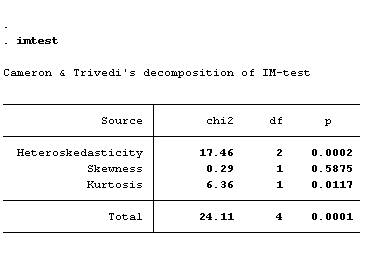
\includegraphics[]{WhiteTestHabit.png}

\end{table}

\begin{table}
\centering
\caption{Breusch-Pagan Test of Heteroskedasticity for Model 3 ($D_{2015}$ and $D_{2014}$)}

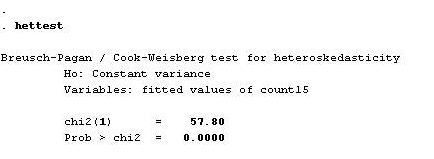
\includegraphics[]{BPTestHabit.png}

\end{table}

\begin{table}
\centering
\caption{White Test of Heteroskedasticity for Model 4 ($D_{2015}$ and $\rho_0$)}

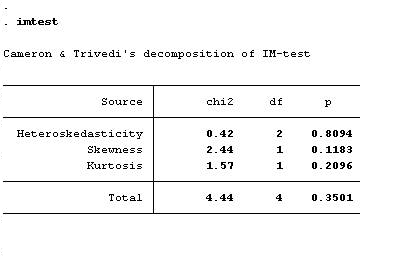
\includegraphics[]{WhiteTestLearning.png}

\end{table}

\begin{table}
\centering
\caption{Breusch-Pagan Test of Heteroskedasticity for Model 4 ($D_{2015}$ and $\rho_0$)}

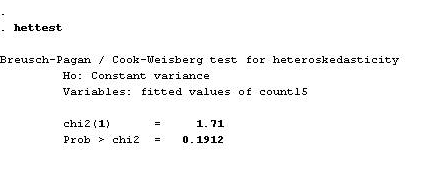
\includegraphics[]{BPTestLearning.png}

\end{table}

\begin{figure}
\caption{Heteroskedasticity of Model 3 (Error term on $D_{2014}$)}
\centering

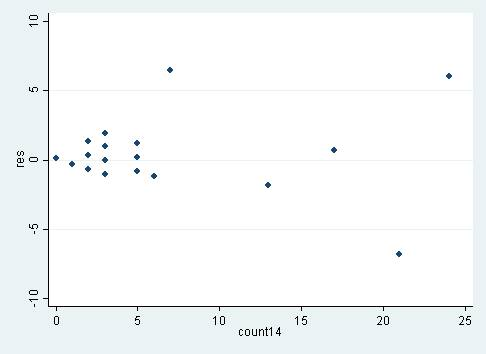
\includegraphics[]{heteroskedasticity_graph.png}
\end{figure}

\begin{figure}
\caption{Heteroskedasticity of Model 4 (Error term on $\rho_0$)}
\centering

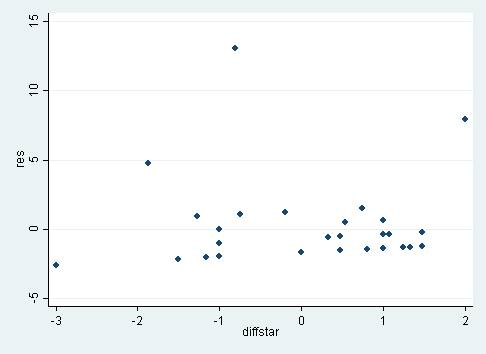
\includegraphics[]{HeteroGraphLearning.png}
\end{figure}
\section{References}

Levy-Garboua, L. and Montmarquette, C. (1996), "A Microeconometric Study of Theatre Demand," \textit{Journal of Cultural Economics} 20: 25-50, 1996.

Becker, G., Grossman, M., and Murphy, K. (1994), "An Empirical Analysis of Cigarette Addiction," \textit{The American Economic Review} Vol. 84, No. 3, pp. 396-418, Jun., 1994.

Becker, G. and Stigler, G. (1977), "De Gustibus Non Est Disputandum," \textit{The American Economic Review} Vol. 67, No. 2, pp. 76-90, Mar., 1977.

Castiglione, C. and Infante, D. (2016), "Rational Addiction and Cultural Goods: The Case of the Italian Theatregoer," \textit{Journal of Cultural Economics}, Volume 40, Issue 2, pp 163-190,  May 2016. 

Davis, D., Dingel, J., Monras, J., and Morales, E. (2016), "How Segregated is Urban Consumption?" Working Paper.

Houthakker, Hendrik S., and Lester D. Taylor. (1970) Consumer Demand in the United States: Analyses and Projections. Cambridge, MA: Harvard UP, 1970. Web.

Pollak, R. (1970), "Habit Formation and Dynamic Demand Functions," \textit{Journal of Political Economy}, Vol: 78, No. 4, pp. 745-63, 1970.

Marrone, J. (forthcoming), "Culture as a Habit: Assimilation and Language
Learning Over the Lifecycle," Working Paper.

Yamamura, E. (2008), "Socio-economic effects on increased cinema attendance: The case of Japan," \textit{Journal of Behavioral and Experimental Economics} Vol: 37, No. 6, pp. 2546-2555, December 2008. 
 


\end{document}
